\pdfminorversion=4
\documentclass[aspectratio=169]{beamer}

\mode<presentation>
{
  \usetheme{default}
  \usecolortheme{default}
  \usefonttheme{default}
  \setbeamertemplate{navigation symbols}{}
  \setbeamertemplate{caption}[numbered]
  \setbeamertemplate{footline}[frame number]  % or "page number"
  \setbeamercolor{frametitle}{fg=white}
  \setbeamercolor{footline}{fg=black}
} 

\usepackage[english]{babel}
\usepackage[utf8x]{inputenc}
\usepackage{tikz}
\usepackage{courier}
\usepackage{array}
\usepackage{bold-extra}
\usepackage{minted}
\usepackage[thicklines]{cancel}
\usepackage{fancyvrb}

\xdefinecolor{dianablue}{rgb}{0.18,0.24,0.31}
\xdefinecolor{darkblue}{rgb}{0.1,0.1,0.7}
\xdefinecolor{darkgreen}{rgb}{0,0.5,0}
\xdefinecolor{darkgrey}{rgb}{0.35,0.35,0.35}
\xdefinecolor{darkorange}{rgb}{0.8,0.5,0}
\xdefinecolor{darkred}{rgb}{0.7,0,0}
\definecolor{darkgreen}{rgb}{0,0.6,0}
\definecolor{mauve}{rgb}{0.58,0,0.82}

\title[2019-05-09-physicsforum-languages]{Analysis Description Languages}
\author{Jim Pivarski}
\institute{Princeton University -- IRIS-HEP}
\date{May 9, 2019}

\usetikzlibrary{shapes.callouts}

\begin{document}

\logo{\pgfputat{\pgfxy(0.11, 7.4)}{\pgfbox[right,base]{\tikz{\filldraw[fill=dianablue, draw=none] (0 cm, 0 cm) rectangle (50 cm, 1 cm);}\mbox{\hspace{-8 cm}
\includegraphics[height=1 cm]{princeton-logo-long.png}\hspace{0.1 cm}\raisebox{0.1 cm}{
\includegraphics[height=0.8 cm]{iris-hep-logo-long.png}}\hspace{0.1 cm}}}}}

\begin{frame}
  \titlepage
\end{frame}

\logo{\pgfputat{\pgfxy(0.11, 7.4)}{\pgfbox[right,base]{\tikz{\filldraw[fill=dianablue, draw=none] (0 cm, 0 cm) rectangle (50 cm, 1 cm);}\mbox{\hspace{-8 cm}
\includegraphics[height=1 cm]{princeton-logo.png}\hspace{0.1 cm}\raisebox{0.1 cm}{
\includegraphics[height=0.8 cm]{iris-hep-logo.png}}\hspace{0.1 cm}}}}}

% Uncomment these lines for an automatically generated outline.
%\begin{frame}{Outline}
%  \tableofcontents
%\end{frame}

% START START START START START START START START START START START START START

\begin{frame}{}
\vspace{-0.25 cm}
\begin{columns}[t]
\column{1.15\linewidth}
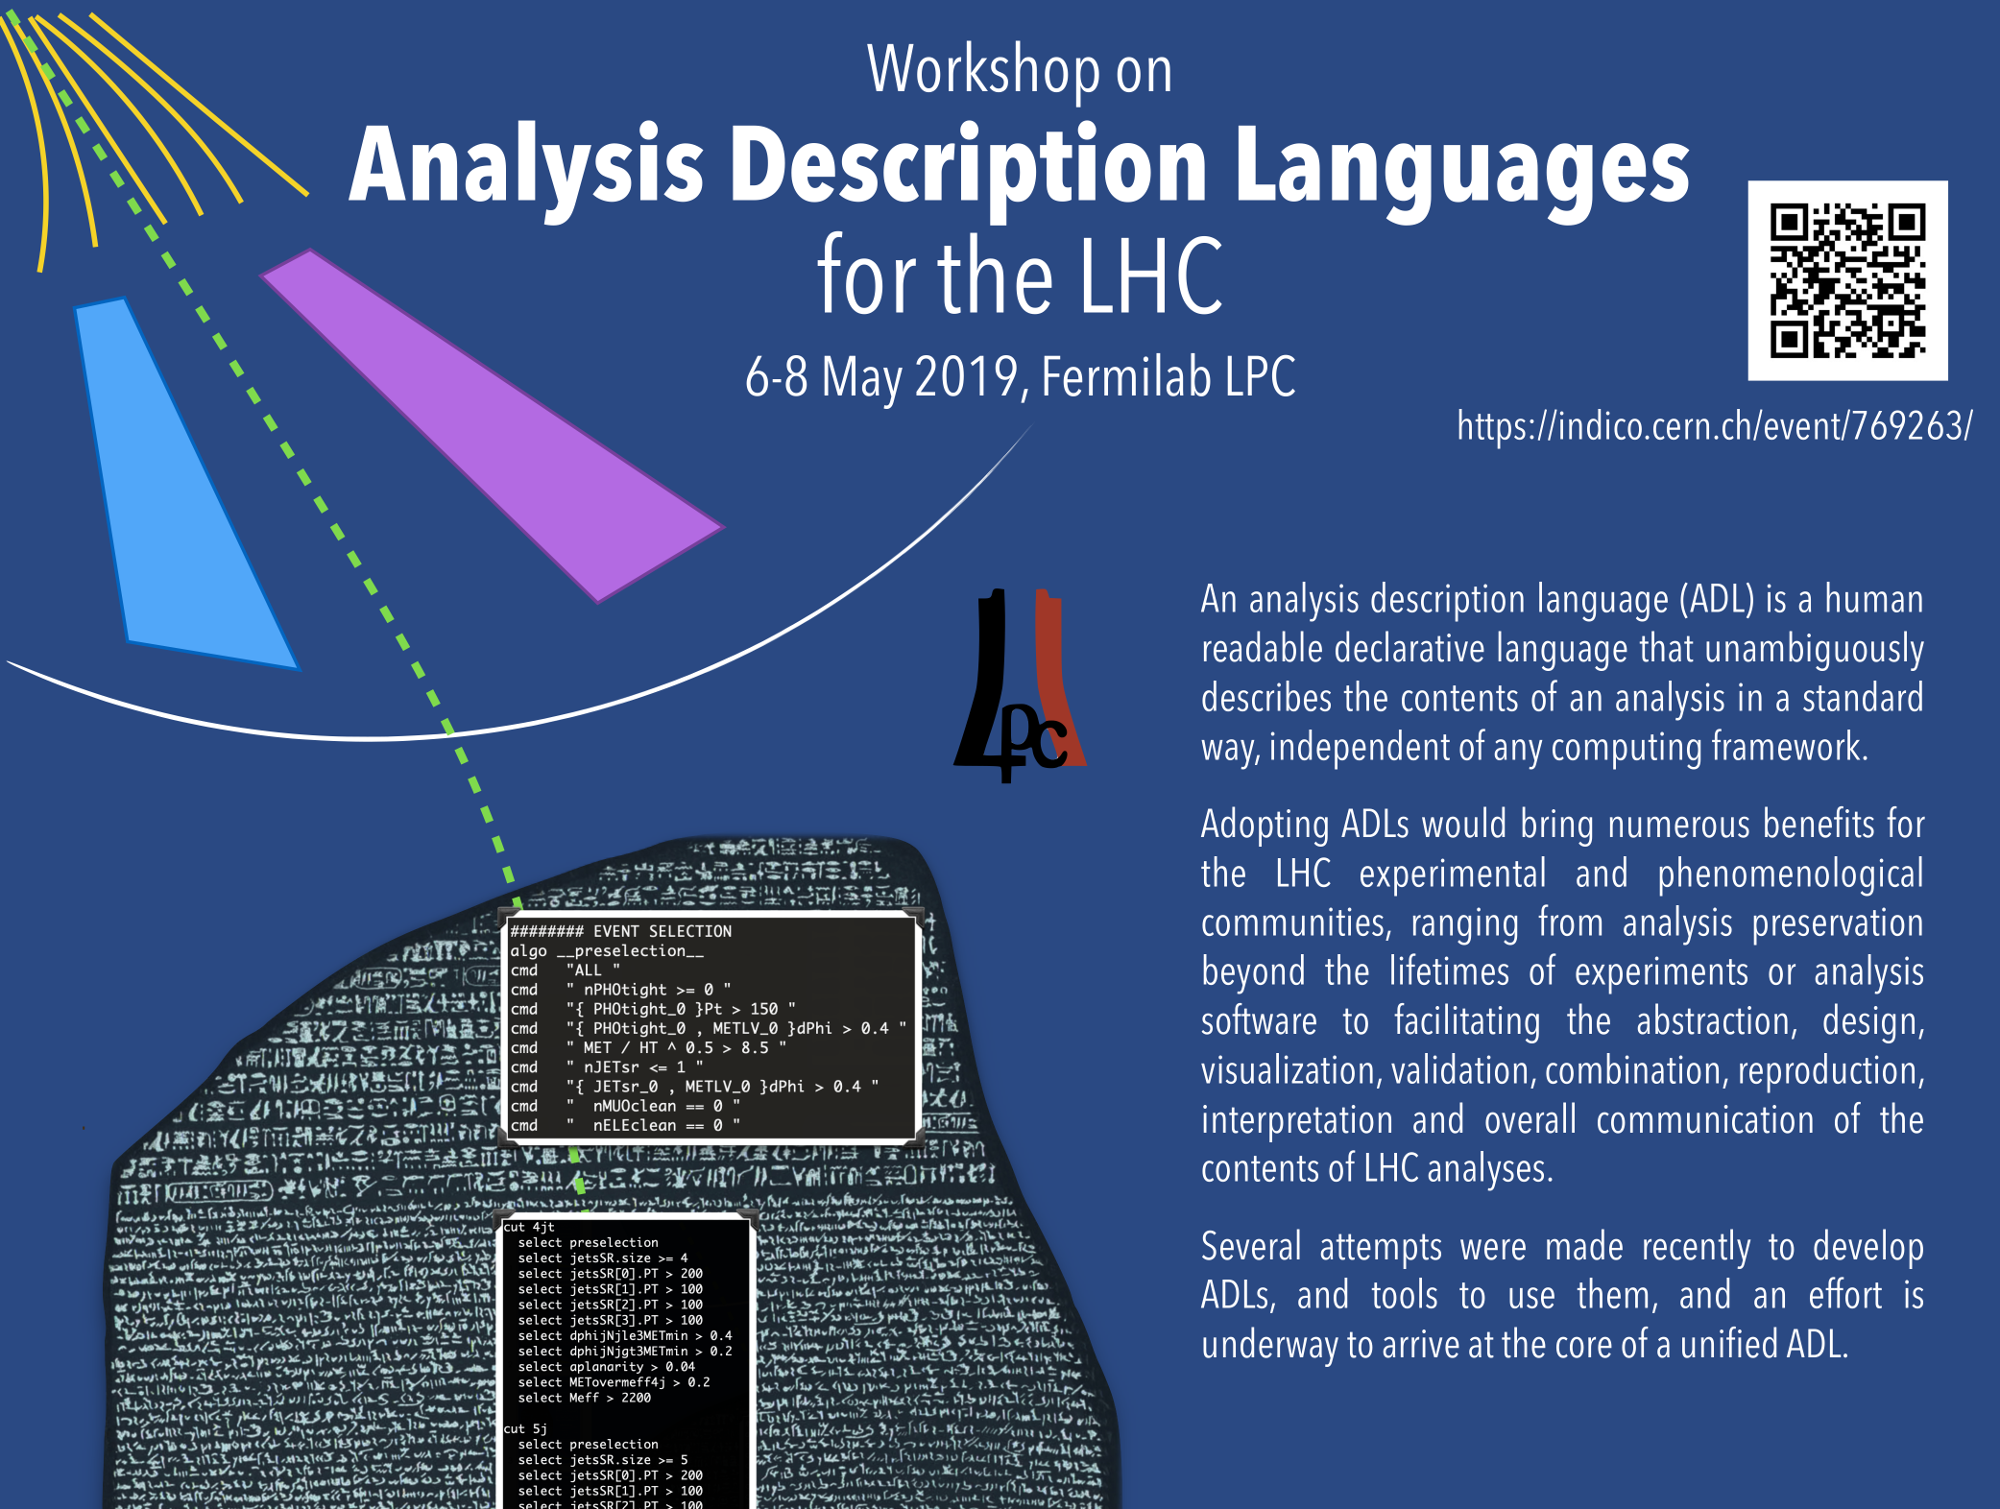
\includegraphics[width=\linewidth]{ADLposter_v3.png}
\end{columns}
\end{frame}

\begin{frame}{What do Analysis Description Languages do?}
\huge
\vspace{0.5 cm}
\begin{center}
\only<1>{Nothing.}\only<2>{They reformulate a computational task in a way that's easier for the analyst to think about.}
\end{center}
\end{frame}

\begin{frame}{Physicists should be aware of the value of abstraction}
\large
\vspace{0.5 cm}
\begin{columns}
\column{0.25\linewidth}
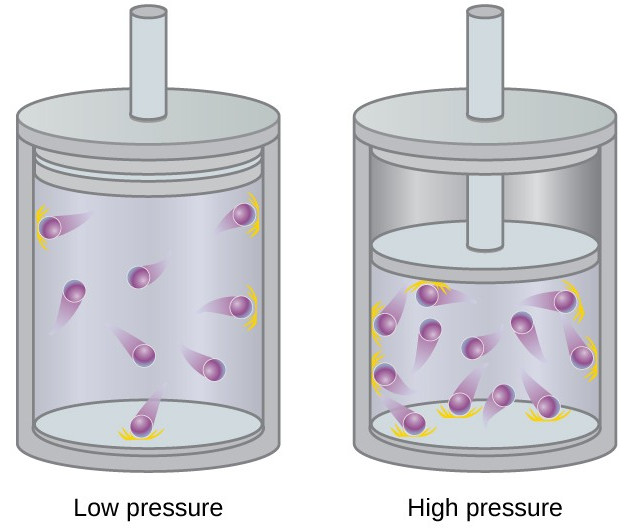
\includegraphics[width=\linewidth]{idealgas.jpg}

\column{0.6\linewidth}
\begin{block}{\LARGE Thermodynamics:}
\vspace{0.1 cm}
Replaces a problem of $\mathcal{O}(10^{24})$ free parameters

\vspace{0.1 cm}
with a problem of $\mathcal{O}(3)$ free parameters.
\end{block}
\end{columns}

\vspace{0.8 cm}
\begin{uncoverenv}<2->
\begin{columns}
\column{0.6\linewidth}
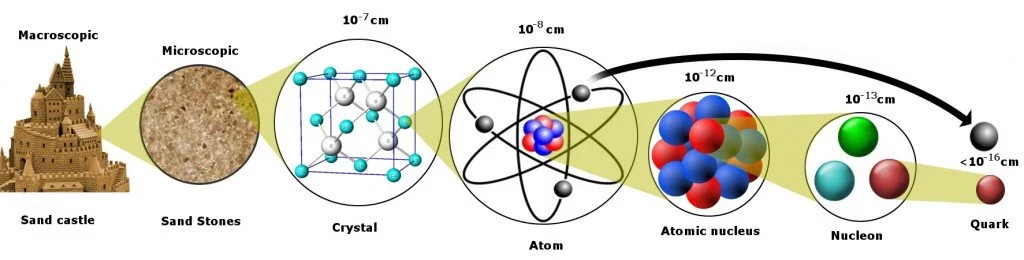
\includegraphics[width=\linewidth]{atom-proton-quark.png}

\column{0.3\linewidth}
\begin{block}{\LARGE Effective theories:}
\vspace{0.2 cm}
Allow you to focus on

\vspace{0.1 cm}
one problem at a time.
\end{block}
\end{columns}
\end{uncoverenv}
\end{frame}

\begin{frame}[fragile]{Much of computer science is about abstracting away details}
\scriptsize
\vspace{0.2 cm}
\begin{minted}{c++}
double bessel_j0(double x) {      // one value goes in...
    double out;
    if (fabs(x) < 8.0) {
        double y = x*x;
        double ans1 = 57568490574.0 + y*(-13362590354.0 + y*(651619640.7
                      + y*(-11214424.18 + y*(77392.33017 + y*(-184.9052456)))));
        double ans2 = 57568490411.0 + y*(1029532985.0 + y*(9494680.718
                      + y*(59272.64853 + y*(267.8532712 + y*1.0))));
        out = ans1 / ans2;
    }
    else {
        double z = 8.0 / fabs(x);
        double y = z*z;
        double xx = fabs(x) - 0.785398164;
        double ans1 = 1.0 + y*(-0.1098628627e-2 + y*(0.2734510407e-4
                      + y*(-0.2073370639e-5 + y*0.2093887211e-6)));
        double ans2 = -0.1562499995e-1 + y*(0.1430488765e-3
                      + y*(-0.6911147651e-5 + y*(0.7621095161e-6
                      - y*0.934935152e-7)));
        out = sqrt(0.636619772/fabs(x))*(cos(xx)*ans1 - z*sin(xx)*ans2);
    }
    return out;                   // ...one value comes out
}
\end{minted}
\end{frame}

\begin{frame}{Smaller numbers of external parameters are easier to think about}
\vspace{0.2 cm}
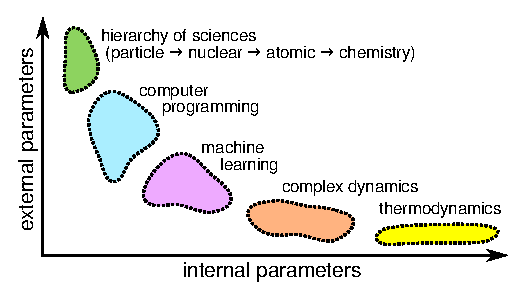
\includegraphics[width=\linewidth]{internal-vs-external.pdf}
\end{frame}



\end{document}
